
\begin{myex}
	Une entreprise étudie ses ventes trimestrielles de paquets de cafés :\\
	
		
	%\centering

	\begin{center}
			{\footnotesize  \begin{tabular}{|@{\ }c@{\ }|@{\ }c@{\ }|@{\ }c@{\ }|@{\ }c@{\ }|@{\ }c@{\ }|@{\ }c@{\ }|@{\ }c@{\ }|}
			\hline
			\multirow{2}{*}{Trimestre}               & \multicolumn{2}{c|}{2008} & \multicolumn{4}{c|}{2009}      \\ \cline{2-7} 
			& $3^e$       & $4^e$       & $1^{er}$ & $2^e$ & $3^e$ & $4^e$ \\ \hline
			Rang $x_i$ du trimestre                  & 1           & 2           & 3      & 4     & 5     & 6     \\ \hline
			Nombre d'unités vendues $y_i$ en millier & 470         & 530         & 550    & 620   & 680   & 660   \\ \hline
		\end{tabular}}
	\end{center}
	
	\vspace*{5mm}
	
	\begin{multicols}{2}
			\begin{itemize}
				\item La moyenne des abscisses est : $\bar{x} = 3,5$;
				\item La moyenne des ordonnées est : $\bar{y} = 585$
				\item Les coordonnées du point moyen G sont donc : $(3,5 ; 585)$.\\
			\end{itemize}
			
			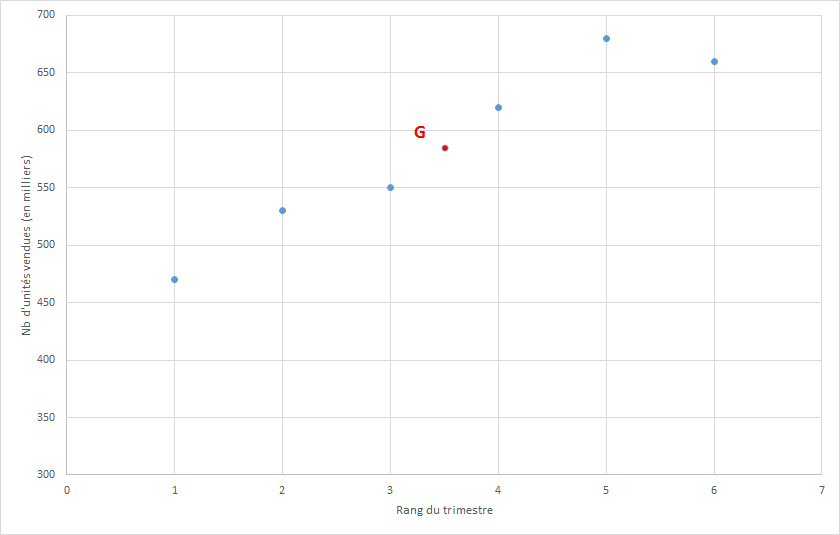
\includegraphics[scale=0.5]{./img/graph}
	\end{multicols}

\end{myex}